\documentclass[12pt]{scrartcl}

\usepackage[utf8]{inputenc}
\usepackage[naustrian]{babel}
\usepackage{caption}
\usepackage{graphicx}
\usepackage{verbatim}
\usepackage[T1]{fontenc}
\usepackage{lmodern}
\usepackage{subcaption}
\usepackage{amsmath}
\usepackage{amsfonts}
\usepackage{listings}
\usepackage{float}
\usepackage{tikz}

%pdfs
\usepackage{pdfpages}
\usepackage{tikz}

%page borders
\usepackage{geometry}
\geometry{left=2.5cm,right=2.5cm,top=3cm,bottom=2.5cm}

\usepackage{minted}
\setminted {
	%style=igor, %borland, autumn, vs
	encoding=utf-8,
	autogobble,
	tabsize=4,
	linenos,
	breaklines,
	keywordcase=upper,
	%escapeinside=||
	%bgcolor=bg
	%frame=single
}

\newenvironment{code}{\captionsetup{type=listing}}{}

%title/footer/header values
\usepackage{titling}
\title{DES3UE Übung 6}
\author{Elias Leonhardsberger}
\date{\today{}, Hagenberg}

%footer/header
%\usepackage[automark]{scrpage2}
%\pagestyle{headings}
%\clearscrheadfoot
%\ihead{\thetitle}
%\chead{\theauthor}
%\ohead{\today}
%\cfoot{Seite \pagemark}

\begin{document}
\clearpage
\thispagestyle{empty}
\begin{tikzpicture}[remember picture, overlay]
	\node at (current page.center) {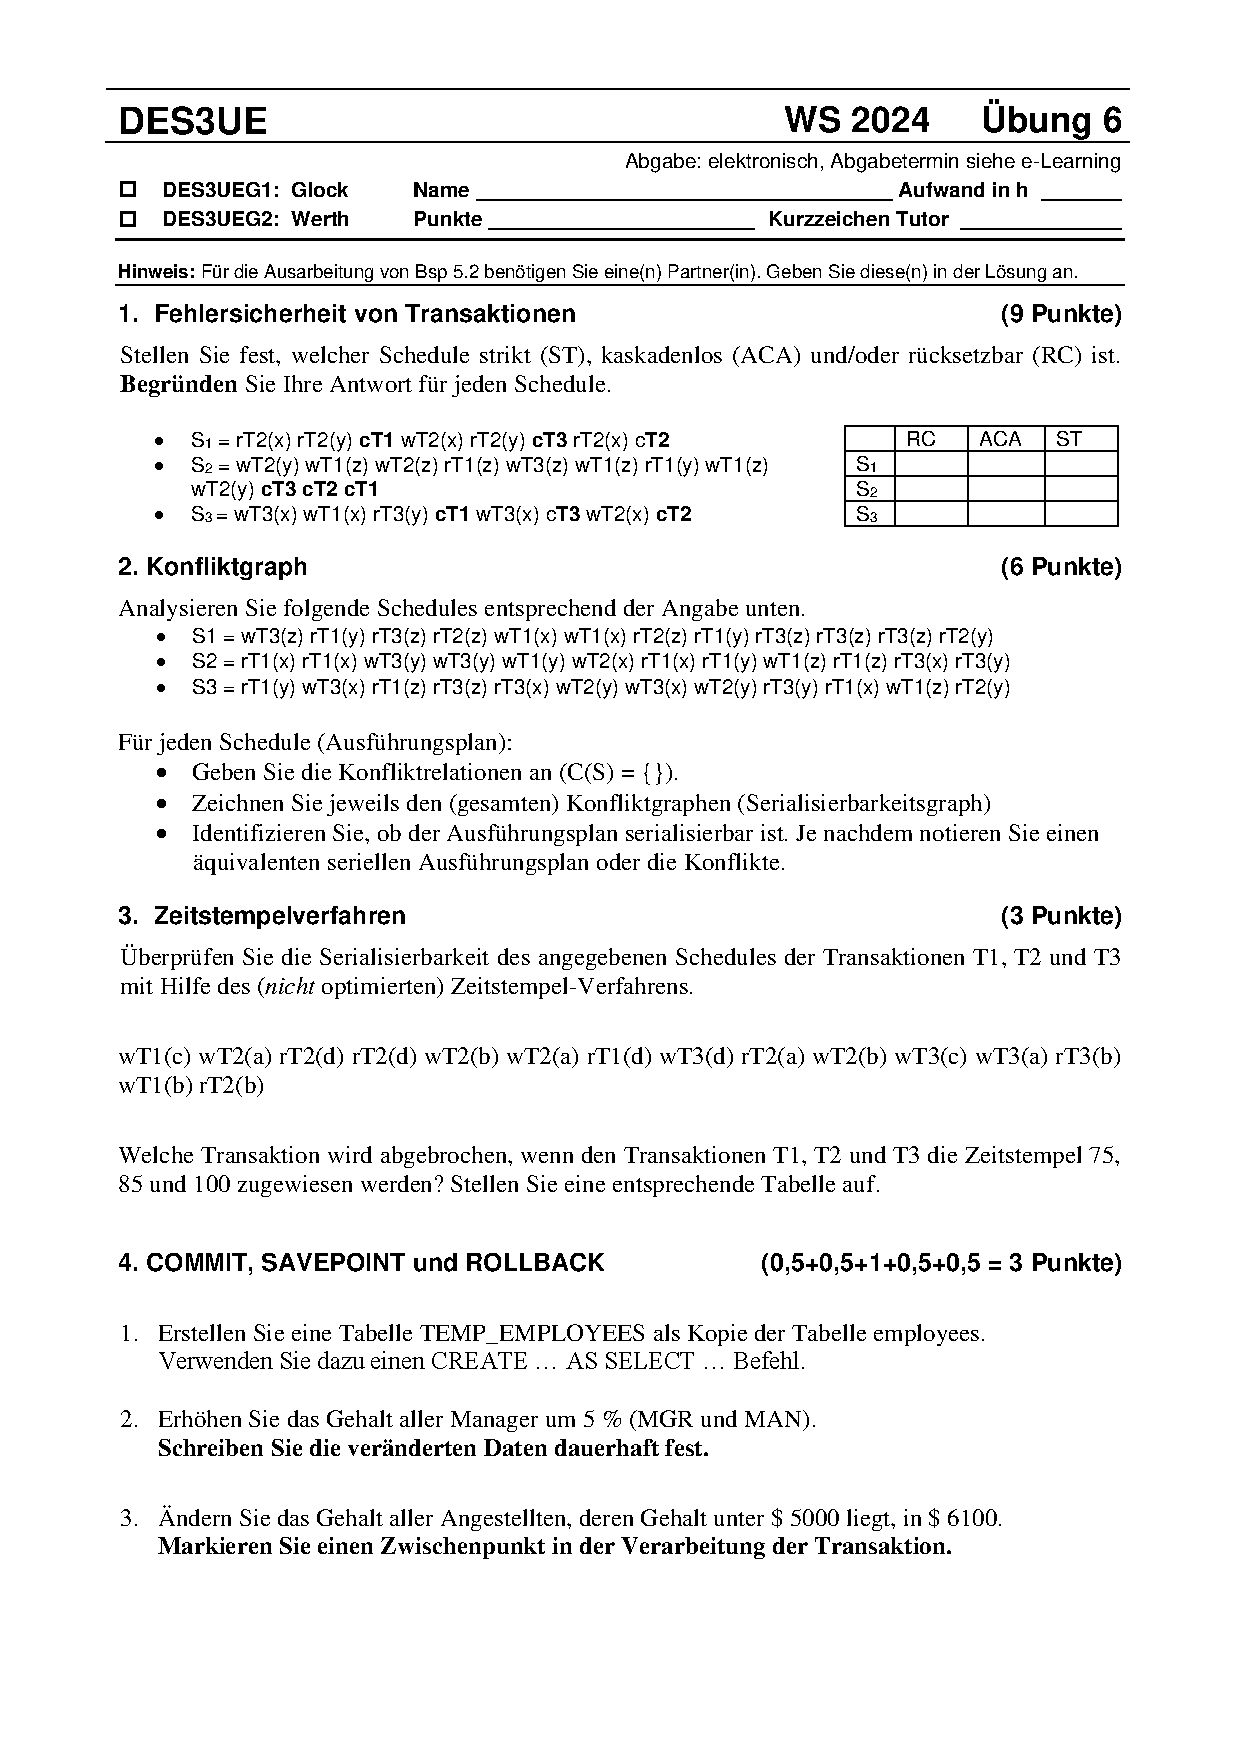
\includegraphics[page=1]{Angabe.pdf}};
	\begin{scope}[shift={(current page.south west)},every node/.style={anchor=base west}]
		\node at (1.87cm, 26.33cm) {X};
		\node at (8.0cm, 26.4cm) {\theauthor};
		\node at (17.7cm, 26.4cm) {2};
	\end{scope}
\end{tikzpicture}

\includepdf[pages=2-3]{Angabe.pdf}

\maketitle
\tableofcontents

\pagebreak

\section{Fehlersicherheit vor Transaktionen}

\begin{center}
	\begin{tabular}{ | c | c | c | c | }
		\hline
		      & RC & ACA & ST \\
		\hline
		$S_1$ & X  & X   & X  \\
		\hline
		$S_2$ &    &     &    \\
		\hline
		$S_3$ & X  & X   &    \\
		\hline
	\end{tabular}
\end{center}

\subsection{$S_1$}

\begin{center}
	\begin{tabular}{ | c | c | }
		\hline
		x   & y                       \\
		\hline
		rT2 & rT2                     \\
		\multicolumn{2}{ | c | }{cT1} \\
		wT2 & rT2                     \\
		\multicolumn{2}{ | c | }{cT3} \\
		rT2 &                         \\
		\multicolumn{2}{ | c | }{cT2} \\
		\hline
	\end{tabular}
\end{center}

$S_1$ ist strikt seriell da nur T2 liest und schreibt. Da es strikt ist, ist es auch kaskadenlos und rücksetzbar.

\subsection{$S_2$}

\begin{center}
	\begin{tabular}{ | c | c | }
		\hline
		y   & z                       \\
		\hline
		wT2 & wT1                     \\
		rT1 & wT2                     \\
		    & rT1                     \\
		    & wT3                     \\
		    & wT1                     \\
		    & wT1                     \\
		    & wT2                     \\
		\multicolumn{2}{ | c | }{cT3} \\
		\multicolumn{2}{ | c | }{cT2} \\
		\multicolumn{2}{ | c | }{cT1} \\
		\hline
	\end{tabular}
\end{center}

$S_2$ hat keine der gefragten Eigenschaften, da T1 vor T2 schreibt und nach T2 liest.

\subsection{$S_3$}

\begin{center}
	\begin{tabular}{ | c | c | }
		\hline
		x   & y                       \\
		\hline
		wT3 & rT3                     \\
		wT1 &                         \\
		\multicolumn{2}{ | c | }{cT1} \\
		wT3 &                         \\
		\multicolumn{2}{ | c | }{cT3} \\
		wT2 &                         \\
		\multicolumn{2}{ | c | }{cT2} \\
		\hline
	\end{tabular}
\end{center}

$S_3$ ist kaskadenlos da kein Lesevorgang nach einem uncommiteten Schreibvorgang stattfindet.
Es ist auch rücksetzbar da es kaskadenlos ist. Es ist jedoch nicht fehlerfrei serialisierbar.

\section{Konfliktgraph}

\subsection{$S_1$}

\begin{center}
	\begin{tabular}{ | c | c | c | }
		\hline
		x   & y   & Z   \\
		\hline
		wT1 & rT1 & wT3 \\
		wT1 & rT1 & rT3 \\
		    & rT2 & rT2 \\
		    &     & rT2 \\
		    &     & rT3 \\
		    &     & rT3 \\
		    &     & rT3 \\
		\hline
	\end{tabular}
\end{center}

\begin{align*}
	C(S_1) = \{ rw_z(T3, T2) \}
\end{align*}

\begin{center}
	\begin{tikzpicture}[node distance={30mm}, main/.style = {draw, circle}]
		\node[main] (1) {T1};
		\node[main] (2) [below right of=1] {T2};
		\node[main] (3) [below left of=1] {T3};

		\draw[->] (3) edge [bend left=0] node[midway, above, sloped, pos=0.5] {wr z} (2);
	\end{tikzpicture}
\end{center}

$S_1$ ist konfliktserialisierbar, da kein Zyklus im Graphen existiert.

\subsection{$S_2$}

\begin{center}
	\begin{tabular}{ | c | c | c | }
		\hline
		x   & y   & Z   \\
		\hline
		rT1 & wT3 & wT1 \\
		rT1 & wT3 & rT1 \\
		wT2 & wT1 &     \\
		rT1 & rT1 &     \\
		rT3 & rT3 &     \\
		\hline
	\end{tabular}
\end{center}

\begin{align*}
	C(S_2) = \{ rw_x(T1, T2), wr_x(T2, T1), wr_x(T2, T3), ww_y(T3, T1), wr_y(T1, T3) \}
\end{align*}

\begin{center}
	\begin{tikzpicture}[node distance={30mm}, main/.style = {draw, circle}]
		\node[main] (1) {T1};
		\node[main] (2) [below right of=1] {T2};
		\node[main] (3) [below left of=1] {T3};

		\draw[->] (1) edge [bend left=15] node[midway, above, sloped, pos=0.5] {rw x} (2);
		\draw[->] (2) edge [bend left=15] node[midway, above, sloped, pos=0.5] {wr x} (1);
		\draw[->] (2) edge [bend left=0] node[midway, above, sloped, pos=0.5] {wr x} (3);
		\draw[->] (3) edge [bend left=15] node[midway, above, sloped, pos=0.5] {ww y} (1);
		\draw[->] (1) edge [bend left=15] node[midway, above, sloped, pos=0.5] {wr y} (3);
	\end{tikzpicture}
\end{center}

$S_2$ ist nicht konfliktserialisierbar, da ein Zyklus im Graphen existiert.

\pagebreak
\subsection{$S_3$}

\begin{center}
	\begin{tabular}{ | c | c | c | }
		\hline
		x   & y   & Z   \\
		\hline
		wT3 & rT1 & rT1 \\
		rT3 & wT2 & rT3 \\
		wT3 & wT2 & wT1 \\
		rT1 & rT3 &     \\
		    & rT2 &     \\
		\hline
	\end{tabular}
\end{center}

\begin{align*}
	C(S_3) = \{ wr_x(T3, T1), rw_y(T1, T2), wr_y(T2, T3), rw_z(T3, T1) \}
\end{align*}

\begin{center}
	\begin{tikzpicture}[node distance={30mm}, main/.style = {draw, circle}]
		\node[main] (1) {T1};
		\node[main] (2) [below right of=1] {T2};
		\node[main] (3) [below left of=1] {T3};

		\draw[->] (3) edge [bend right=15] node[midway, above, sloped, pos=0.5] {wr x} (1);
		\draw[->] (1) edge [bend left=0] node[midway, above, sloped, pos=0.5] {rw y} (2);
		\draw[->] (2) edge [bend left=0] node[midway, above, sloped, pos=0.5] {wr y} (3);
		\draw[->] (3) edge [bend left=15] node[midway, above, sloped, pos=0.5] {rw z} (1);
	\end{tikzpicture}
\end{center}

$S_3$ ist nicht konfliktserialisierbar, da ein Zyklus im Graphen existiert.

\section{Zeitstempelverfahren}

\begin{center}
	\begin{tabular}{ | c | c | c | c | c | c | c | c | c | c | c | }
		\hline
		75   & 85   & 100  & \multicolumn{2}{ c | }{a} & \multicolumn{2}{ | c | }{b} & \multicolumn{2}{ | c | }{c} & \multicolumn{2}{ | c | }{d}                             \\
		\hline
		T1   & T2   & T3   & R(a)                      & W(a)                        & R(b)                        & W(b)                        & R(c) & W(c) & R(d) & W(d) \\
		\hline
		w(c) &      &      &                           &                             &                             &                             & 75   & 75   &      &      \\
		     & w(a) &      & 85                        & 85                          &                             &                             & 75   & 75   &      &      \\
		     & r(d) &      & 85                        & 85                          &                             &                             & 75   & 75   & 85   &      \\
		     & r(d) &      & 85                        & 85                          &                             &                             & 75   & 75   & 85   &      \\
		     & w(b) &      & 85                        & 85                          & 85                          & 85                          & 75   & 75   & 85   &      \\
		     & w(a) &      & 85                        & 85                          & 85                          & 85                          & 75   & 75   & 85   &      \\
		r(d) &      &      & 85                        & 85                          & 85                          & 85                          & 75   & 75   & 85   &      \\
		     &      & w(d) & 85                        & 85                          & 85                          & 85                          & 75   & 75   & 85   & 100  \\
		     & r(a) &      & 85                        & 85                          & 85                          & 85                          & 75   & 75   & 85   & 100  \\
		     & w(b) &      & 85                        & 85                          & 85                          & 85                          & 75   & 75   & 85   & 100  \\
		     &      & w(c) & 85                        & 85                          & 85                          & 85                          & 100  & 100  & 85   & 100  \\
		     &      & w(a) & 100                       & 100                         & 85                          & 85                          & 100  & 100  & 85   & 100  \\
		     &      & r(b) & 100                       & 100                         & 85                          & 85                          & 100  & 100  & 85   & 100  \\
		w(b) &      &      & 100                       & 100                         & 85                          & x                           & 100  & 100  & 85   & 100  \\
		     & r(b) &      & 100                       & 100                         & 85                          & x                           & 100  & 100  & 85   & 100  \\
		\hline
	\end{tabular}
\end{center}

T1 versucht auf b zu schreiben nachdem T2 beteits auf b geschrieben hat. T1 wird deshalb abgebrochen.

\pagebreak

\section{COMMIT, SAVEPOINT und ROLLBACK}

\subsection{SQL Statements}
\inputminted{sql}{../ue6_4.sql}

\pagebreak

\subsection{Ausgabe}

\begin{figure}[H]
	\centering
	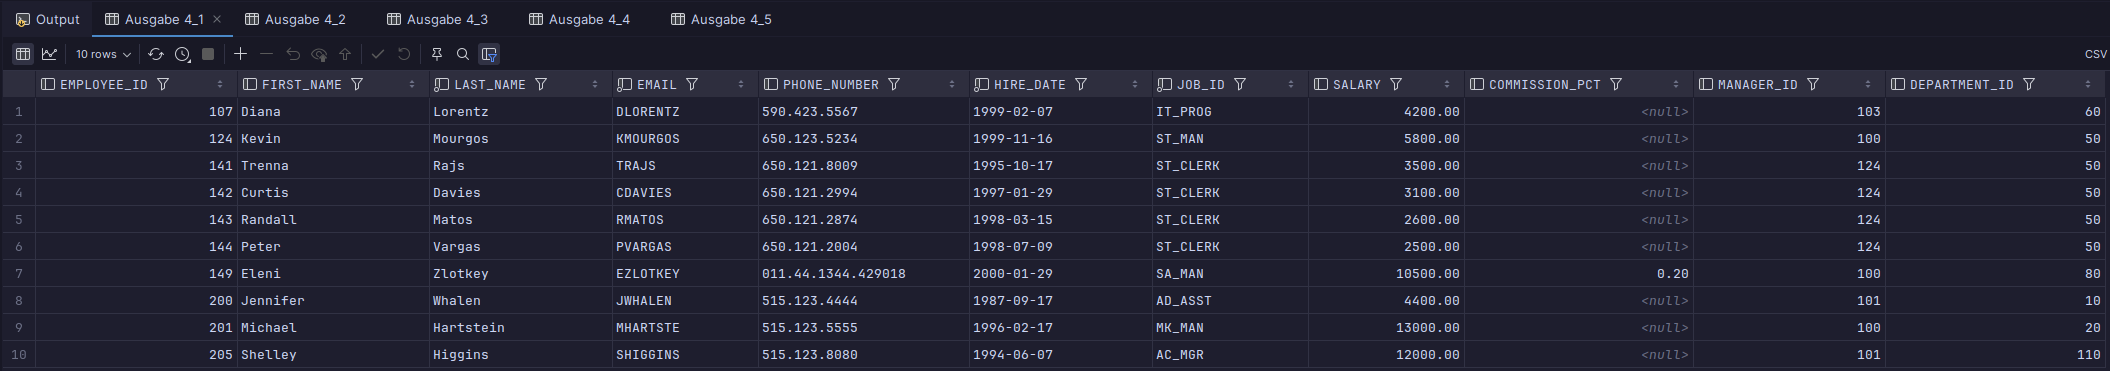
\includegraphics[width=1\textwidth]{../4_1.png}
	\caption{Ausgabe 4\textunderscore1}
\end{figure}

\begin{figure}[H]
	\centering
	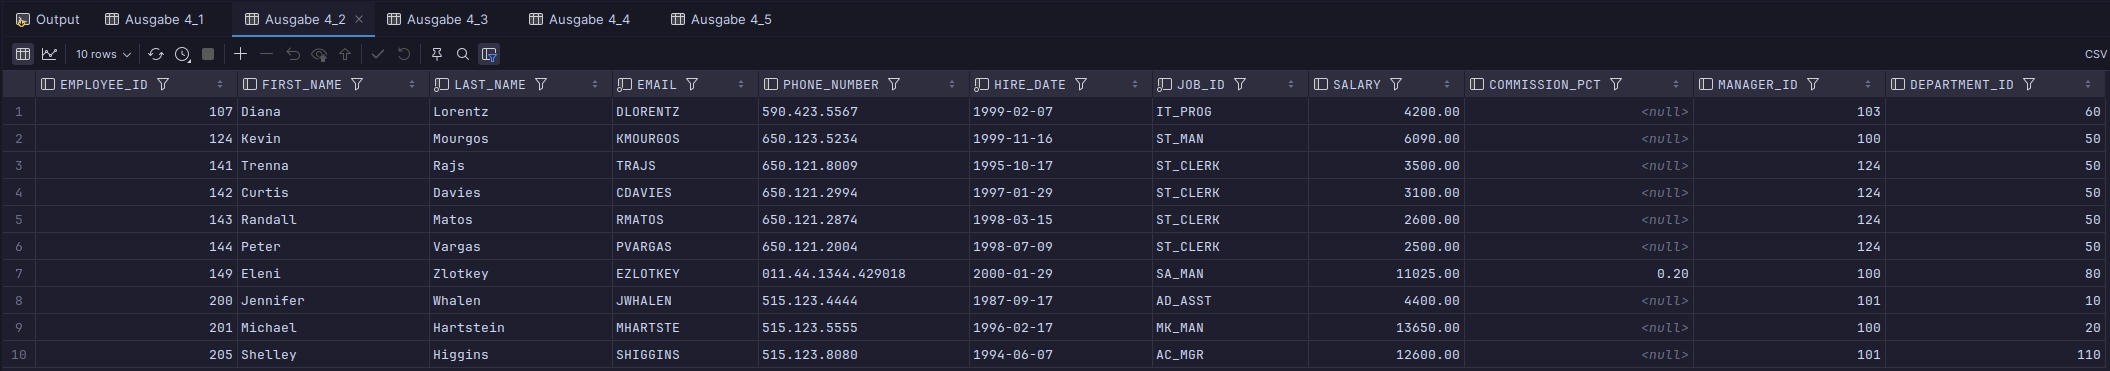
\includegraphics[width=1\textwidth]{../4_2.png}
	\caption{Ausgabe 4\textunderscore2}
\end{figure}

\begin{figure}[H]
	\centering
	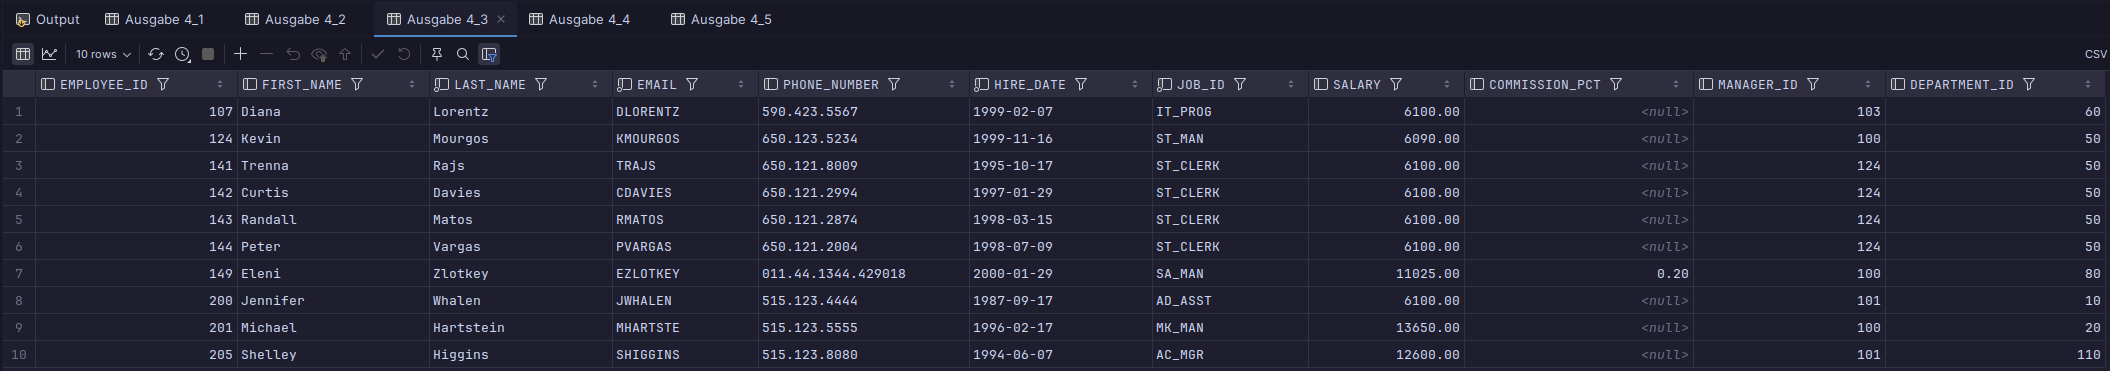
\includegraphics[width=1\textwidth]{../4_3.png}
	\caption{Ausgabe 4\textunderscore3}
\end{figure}

\begin{figure}[H]
	\centering
	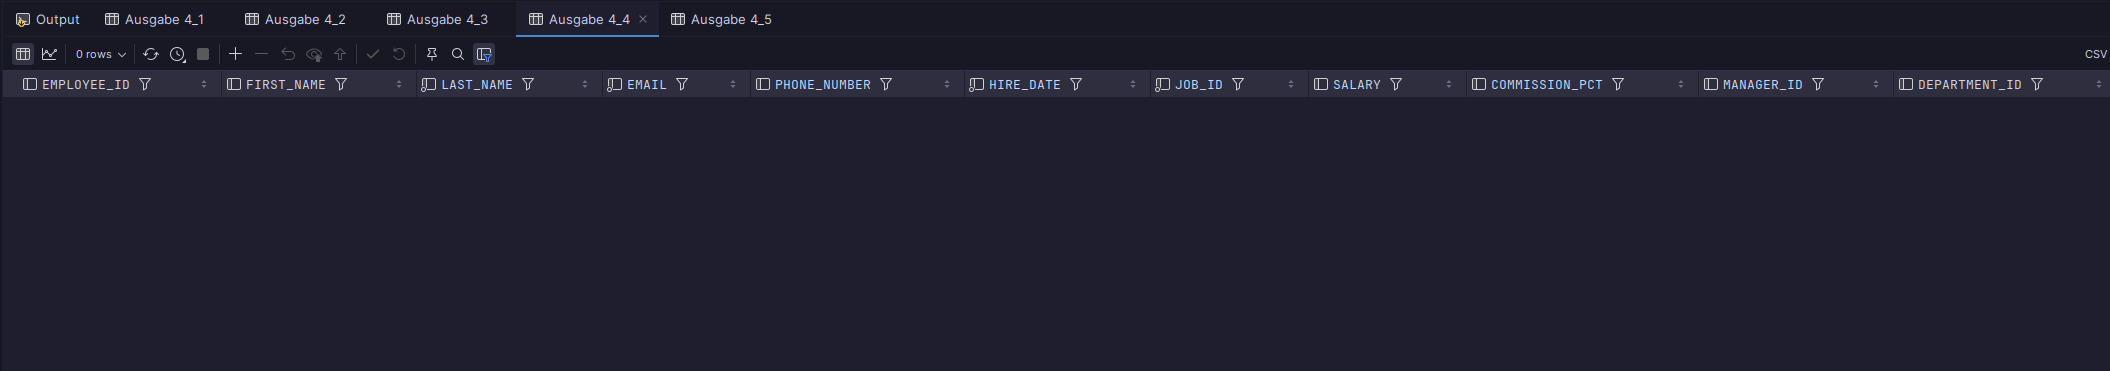
\includegraphics[width=1\textwidth]{../4_4.png}
	\caption{Ausgabe 4\textunderscore4}
\end{figure}

\begin{figure}[H]
	\centering
	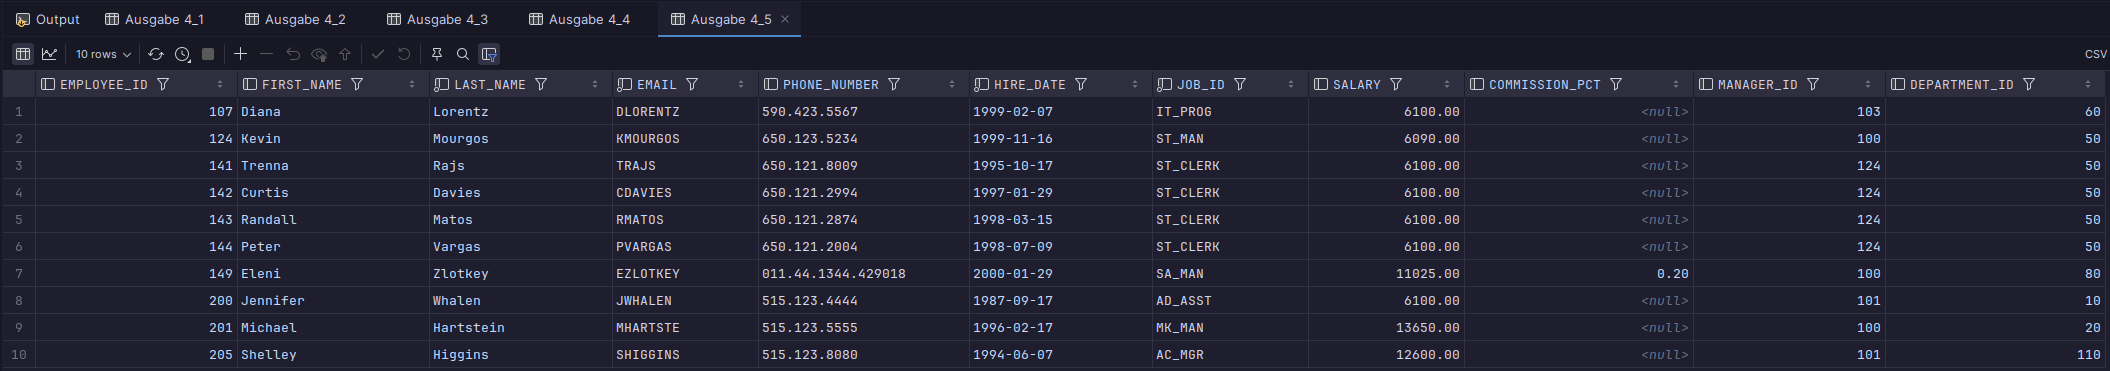
\includegraphics[width=1\textwidth]{../4_5.png}
	\caption{Ausgabe 4\textunderscore5}
\end{figure}

\pagebreak

\section{Vergabe und Entzug von Rechten}

\subsection{SQL Statements}
\inputminted{sql}{../ue6_5.sql}

\subsection{Ausgabe}

\begin{figure}[H]
	\centering
	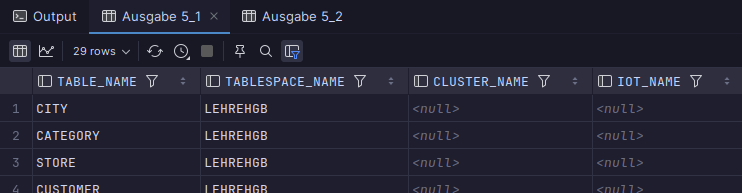
\includegraphics[width=0.6\textwidth]{../5_1.png}
	\caption{Ausgabe 5\textunderscore1}
\end{figure}

\begin{figure}[H]
	\centering
	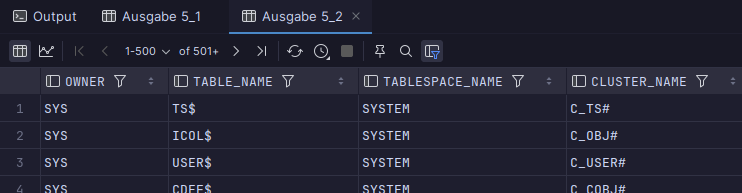
\includegraphics[width=0.6\textwidth]{../5_2.png}
	\caption{Ausgabe 5\textunderscore2}
\end{figure}

Aufgabe 5.2 wurde nicht gemacht.

\section{Zusatzaufgabe}

\begin{center}
	\begin{tabular}{ c | c }
		Angabe & Lösung \\
		\hline
		a      & 2      \\
		b      & 3      \\
		c      & 2      \\
	\end{tabular}
\end{center}

\end{document}